\documentclass{article}
\usepackage{lmodern}
\usepackage{tikz}
\usetikzlibrary{calc}
\pagestyle{empty}
\begin{document}
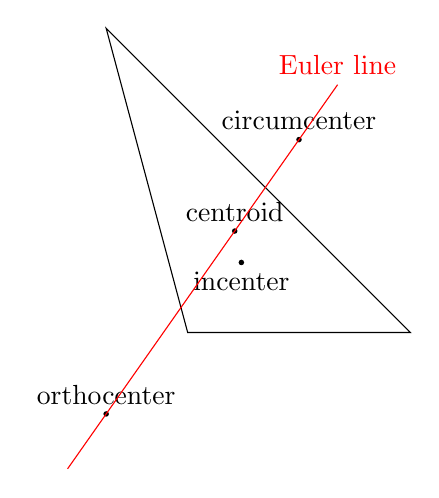
\begin{tikzpicture}
    \coordinate (A) at (0,0);
    \coordinate (B) at (0:{2cm*sqrt(2)});
    \coordinate (C) at (105:4cm);
    \draw (A) -- (B) -- (C) -- cycle;
    \fill (barycentric cs:A=1,B=1,C=1)
        circle[radius=1pt]
        node[above] {centroid};
    \fill (barycentric cs:A={tan(105)},B={tan(45)},C={tan(30)})
        coordinate (H)
        circle[radius=1pt]
        node[above] {orthocenter};
    \fill (barycentric cs:A={sin(210)},B={sin(90)},C={sin(60)})
        coordinate (O)
        circle[radius=1pt]
        node[above] {circumcenter};
    \fill (barycentric cs:A={2+2*sqrt(3)},B=4,C={2*sqrt(2)})
        circle[radius=1pt]
        node[below] {incenter};
    \draw[red] ($(H)!-.2!(O)$) -- ($(H)!1.2!(O)$)
        node[above] {Euler line};
\end{tikzpicture}
\end{document}